\chapter{Implementation}
After providing an analysis of UIProtocol, settling down on the requirements and working out the design of the app, we can now present how the application was being developed, what technologies were used, what problems were encountered and how they were tackled.\\

\subsubsection{Development Environment}
As previously said, the application was written in the Visual Studio 2013 IDE and using C\#, a modern programming language developed by Microsoft. The reasons for choosing Visual Studio (VS) are clear: VS is the main development tool for the whole .NET platform, fully supports C\# and Windows Phone development and debugging. VS is therefore the main tool to be used for most .NET development.\\The programming was backed up by running the code directly on a Windows Phone 8 device, namely HTC 8S. ReSharper

\subsubsection{Overview of Core Classes}
In this section, we will cover the most important classes of the application, to give a brief idea of how the UIP documents are handled, stored, processed and how the UI is rendered. There are several tables in the following pages, illustrating how inner UIP Document representation is stored (Table \ref{tab:uipDocClasses}), how rendering functions (Table \ref{tab:uipRenderClasses}) and how the communication with the server is handled \ref{tab:uipCommClasses}. Apart from the classes mentioned in the tables, there is a number of other helper classes.


\begin{table}[htbp]
  \centering
  \caption{UIP Document Representation Classes}
  \label{tab:uipDocClasses}
 \renewcommand{\arraystretch}{1.2}
    \begin{tabularx}{\textwidth}{p{2.5cm}|X}
    \rowcolor{mygray}
    \textbf{Class Name} & \textbf{Class Description} \\
       Interface & This class represents the UIP interface as a container for more UI elements. This class has its own position, a container and can be embedded into another interface, as specified in Listing \ref{uipInterface}. \\ \hline
       Container & This is the class that stores the information about the particular UI elements. A Container can contain other Containers and instances of Element class.\\ \hline
       Element & Class representing particular UI elements such as button, textfield and more. \\
    \end{tabularx}%
    \label{tab:uipDocClasses2}
\end{table}%

\begin{table}[htbp]
  \centering
  \caption{Classes ensuring the rendering of UI elements}
  \label{tab:uipRenderClasses}
 \renewcommand{\arraystretch}{1.2}
    \begin{tabularx}{\textwidth}{p{3cm}|X}
    \rowcolor{mygray}
    \textbf{Class name} & \textbf{Class description} \\
       Renderer & The main class responsible for rendering the elements stored in the classes of table \ref{tab:uipDocClasses}. Its rendering method walks through the tree structure of UIP Document and invokes rendering of each element. It also does the graceful degradation of unsupported elements. \\ \hline
       IRenderable & An interface which defines methods for acquiring class, style, position and other properties of UIP elements. It is implemented by all classes in table \ref{tab:uipDocClasses}. \\ \hline
       \hspace{0pt}IRenderableContainer & Extension of \texttt{IRenderable} interface. It provides support for layouts and is implemented by instances of Interface and Container. \\
    \end{tabularx}%
\end{table}%

\begin{table}[htbp]
  \centering
  \caption{UIP Server connection classes}
  \label{tab:uipCommClasses}
 \renewcommand{\arraystretch}{1.2}
    \begin{tabularx}{\textwidth}{p{3cm}|X}
    \rowcolor{mygray}
    \textbf{Class name} & \textbf{Class description} \\
      UipConnection & Initiates the connection and is responsible for sending events to the server and processing its responses. Does basic XML validation. \\ \hline
       SocketWorker & Handles the socket communication with UIP server. Sends events and runs a separate thread for receiving server's responses. \\ \hline
       HttpConncetion & Class responsible for acquiring resources via HTTP.
    \end{tabularx}%
\end{table}%

\subsubsection{Communication With UIP Server}
As mentioned in Table \ref{tab:uipCommClasses}, the communication with server in implemented in UipConnection class which exposes its functionality for sending events to the rest of the application - namely the EventManager class. It also is responsible for processing any XML data received from server that is sent to it from a SocketWorker instance.
\\
SocketWorker is the low-level socket communication class which ultimately sends events to the server, such as interface requests or events informing about user actions. It also runs an instance of BackgroundWorker class which, in an extra thread, awaits data from the server. The reason there is a separate thread for receiving data is that we cannot make any assumptions about when the server will send data to the client. Generally speaking, server can decide to send model updates at any time, not only as a response to a certain user action.\\
The communication was observed from another, already implemented client.

\subsubsection{Model Updates and Binding}
Any property of UIP document can, instead of direct value, contain a reference to a model and its property, as described in \ref{subsec:models}. As an example, let us consider a button. The text displayed in the button (its Content) can be either hard-coded into the UIP document or there can be a reference to a model property. If the reference is present, the ModelManager looks into an internally stored dictionary of models and if the model is present, the value of its corresponding property is immediately used. If that is not the case, ModelManager makes a request for the model and once it arrives, its corresponding property's value is used. In both cases, a binding is created so that the future updates of the model property are correctly propagated throughout the application.\\The code which acquires the models and creates binding between model properties and properties of UI elements makes heavy use of asynchronous methods. The async/await operations were introduced with C\# 5.0  and provide a developer with a comfortable way to deal with operations that are potentially blocking. Because requesting and receiving models happens over the internet, it can be considered such. If model request and receive was blocked within a synchronous process, the entire application would be forced to wait. However, by taking advantage of the asynchronous programming, the application continues with other work that doesn't depend on the web resource until the potentially blocking task finishes.

\subsubsection{Interpolations (animations)}
Interpolation allows to move UI controls on the canvas. It is implemented through event which is fired by activating a UI control which is supposed to be interpolated. The server responds by a model update which contains "interpolation" and "duration" attributes. The body of the model update contains the value to which the position will be updated. An example of such model  update is shown in listing 

\lstinputlisting[label=uipInterpolation,caption=UIP model update specifying interpolation]{sources/uipInterpolation.xml}

Both ModelManager and interface manager classes only need to be instantiated once, so that the application state is stored in one place. Therefore ModelManager and InterfaceManager are singleton classes.

\subsubsection{Binding Converters}
It has been said that any property can be bound to a model. However, properties in UIP document can convey a wide range of information - including color, font size, row and column position in grid and etc. Since the model updates are always received as string, the binding has to be provided with a converter (IValueconverter instance) which, considering the given examples, converts the received string to SolidColorBrush, double and integer types, respectively.

\subsubsection{Implementing the UI Element Classes}
When deciding how to represent the platform native components which are displayed to the user, we chose to use wrapper classes which will expose the wrapped object's methods and at the same time be able to set up its properties from the UIP document. All supported native components are therefore wrapped into other classes whose names indicate the enclosed UI element (ie UipButton is a wrapper class of standard Button class). All of these wrapper classes inherit from abstract class UipBase which provides a common support for model binding for all inherited components. This way, adding new UI components with binding support is made easy.
\\The ITextStylable interface is implemented by classes which contain text which can be styled. For example, a UipTextBlock implements this interface in order to be able to set font size, color and more. UipContainer, on the other hand, does not implement it because a container itself does not have anything to style - what about background color?? TODO\\
The figure \ref{fig:UIclasses} shows a class diagram of a few wrapper classes and also ITextStylable being implemented.

\begin{figure}[ht!]
\centering
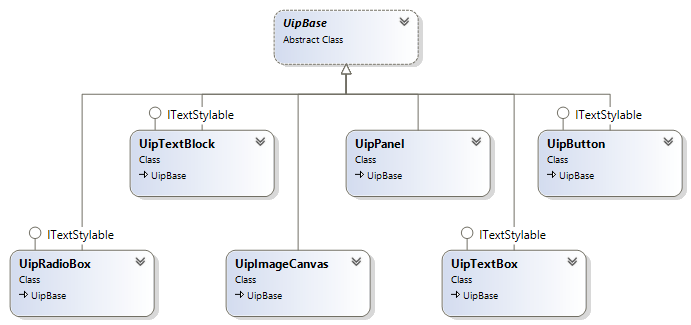
\includegraphics[width=140mm]{pics/UI_classes.png}
\caption{Inheritance tree of several sample UI classes}
\label{fig:UIclasses}
\end{figure}

\subsubsection{Graceful Degradation}
Graceful degradation is a mechanism which replaces unsupported UI elements by supported ones while rendering is being done. This replacement, of course, does not happen without TODO neco jako dan. To illustrate this, let us consider the following example:\\
The server asks the client to render an UIP element of class public.input.choice.single – an UI element known under the WP8 platform as ListPicker (or more generally, a dropdown). This element, however, may not be supported by the client. If this is the case, the graceful degradation takes place and degrades this to public.input.choice which will be rendered as a group of radiobuttons (assuming this basic UI element is supported).

\subsubsection{Event Communication}
Event management is relatively simple: two classes take care of it.



consts class
debugging messages
configuration
interpolation
